\documentclass[a4paper, twocolumn, titlepage, 10pt]{article}
\usepackage{amsmath, graphicx, gensymb, float}
\usepackage{mathtools}
\usepackage{listings}
\usepackage{lettrine}
\usepackage{tabularx}
\title{\textbf{ECSE 307 Linear Systems and Control} \linebreak Lab 4 Report}
\author{Hai XU, 260661832 \and Wenjie WEI, 260685967}
\date{October 25$^{th}$, 2017}
\usepackage{color} %red, green, blue, yellow, cyan, magenta, black, white
\usepackage{inconsolata}
\definecolor{mygreen}{RGB}{28,172,0} % color values Red, Green, Blue
\definecolor{mylilas}{RGB}{170,55,241}

\lstset{language=Matlab,%
	%basicstyle=\color{red},
	basicstyle=\ttfamily,
	breaklines=true,%
	morekeywords={matlab2tikz},
	keywordstyle=\color{blue},%
	morekeywords=[2]{1}, keywordstyle=[2]{\color{black}},
	identifierstyle=\color{black},%
	stringstyle=\color{mylilas},
	commentstyle=\color{mygreen},%
	showstringspaces=false,%without this there will be a symbol in the places where there is a space
	numbers=left,%
	numberstyle={\tiny \color{black}},% size of the numbers
	numbersep=9pt, % this defines how far the numbers are from the text
	emph=[1]{for,end,break},emphstyle=[1]\color{red}, %some words to emphasise
	%emph=[2]{word1,word2}, emphstyle=[2]{style},    
}

\begin{document}
	\maketitle
	\section{Introduction}
		\lettrine{T}{his} lab introduces the methodologies to analyze the behavior of a dynamic system. Proportional, Integral, and Derivative (PID) controls are so far the most common type of controllers that are used. They are simple yet still able to give promising performance. Figure \ref{PIDData} shows what will happen if a PID controller is implemented.
		\begin{figure}[H]
			\centering
			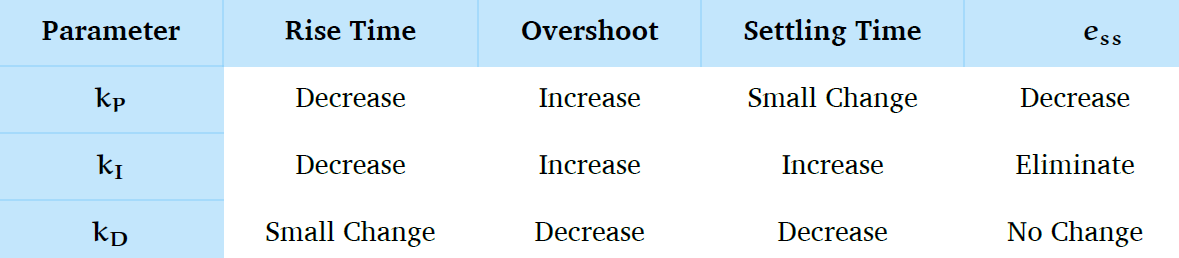
\includegraphics[width=\linewidth]{PIDData}
			\caption{Key Changes that PID Systems Can Bring}
			\label{PIDData}
		\end{figure}
	\section{Finding the PID Gains}
		Consider a system transfer function as below:
		$$
			G(s) = \frac{1}{(s+1)(s+2)(s+3)}
		$$
		Plot the step response using MATLAB. The step response of the system is shown in Figure \ref{G_step}:
		\begin{figure}[H]
			\centering
			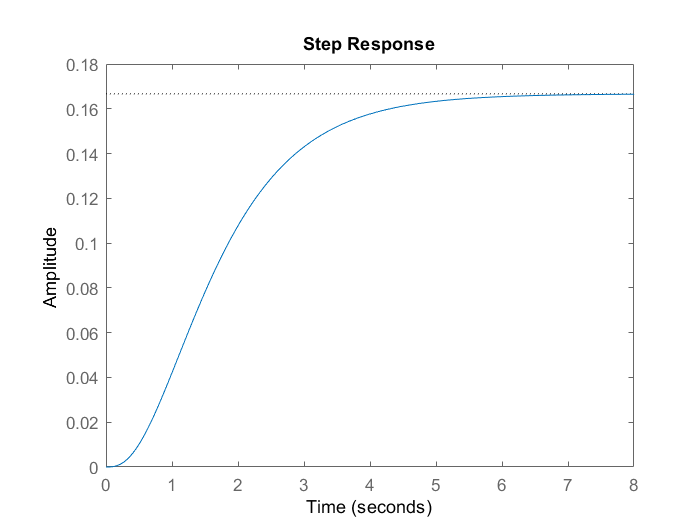
\includegraphics[width=\linewidth]{G_step}
			\caption{Step Response of System G(s)}
			\label{G_step}
		\end{figure}
		
		Apply the MATLAB command:
		\begin{lstlisting}[frame = single]
	stepinfo(G);
		\end{lstlisting}
		A vector containing some critical values will be generated. Table \ref{trtsmptable} shows the most critical data for future analysis of the system:
		\begin{table}[H]
			\centering
			\begin{tabular}{c c c c}
				$e_{ss}$ & $t_r$ & $t_s$ & $M_p$ \\
				 & 2.7428 & 5.0039 & 0
			\end{tabular}
			\caption{Table of Some Critical Values}
			\label{trtsmptable}
		\end{table}
		
		Next, the root locus plot will be needed to explore the stability of the system if we change the gain of the system.
		\begin{figure}[H]
			\centering
			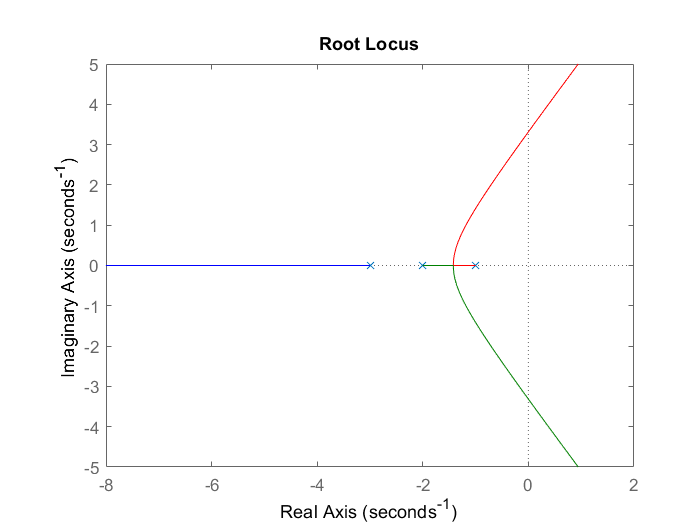
\includegraphics[width=\linewidth]{rlocus}
			\caption{Root-Locus Plot of the System}
			\label{rlocusG}
		\end{figure}
		
		Figure \ref{rlocusG} shows the root locus plot of the system G(s). From the MATLAB plot, we can find that at the marginal stability, gain $K = 60$ and frequency $\omega = 3.31 rad/s$.
		
		Using the information above, we are able to design a stable system with a proper gain. However, as can be seen from Table \ref{trtsmptable}, the rising time $t_r$ is really large, which means that this system responds slowsly to input signals. Idealy, we would like to design a controller that reduces the rise time, settling time, and eliminates the steady-state error. According to Figure \ref{PIDData}, a proportional controller decreases the rising time, and reduces the steady state error as well. Add a proportional controller by implementing the MATLAB code in the Section 3.2 of the Appendix, and find the step response characteristics for $k_p = 40$.
		\begin{figure}[H]
			\centering
			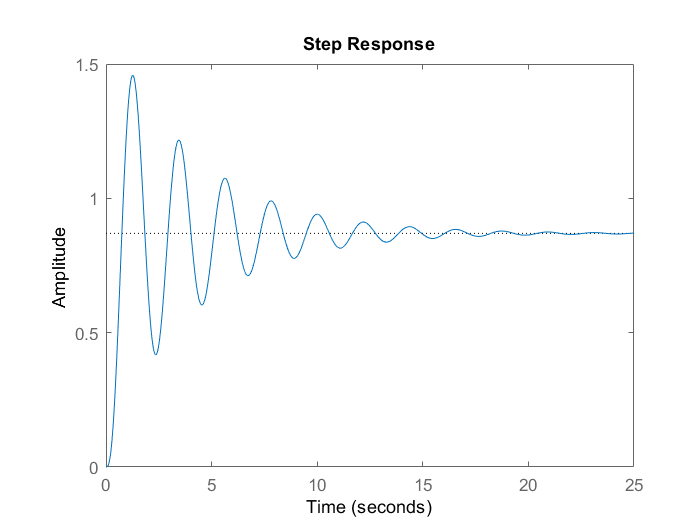
\includegraphics[width=\linewidth]{StepPC}
			\caption{Step Response of the P-Controller}
			\label{steppc}
		\end{figure}
		
		Figure \ref{steppc} shows the step response and Table shows the key response characteristics of the system after adding a proportional controller. 
		\begin{table}[H]
			\centering
			\begin{tabular}{c c c c}
				$e_{ss}$ & $t_r$ & $t_s$ & $M_p$ \\
				& 0.4368 & 15.6105 & 67.6273
			\end{tabular}
			\caption{Table of the Key Characteristics of the P-Controller}
			\label{responseCharPC}
		\end{table}
		
		Compare the data in Table \ref{responseCharPC} and \ref{trtsmptable}, it can be seen clearly that by adding the P-Controller, the system is responding to an input signal much faster. However, the giant overshoot of this system makes the system not as stable as it was before, and the settling time becomes much longer meaning that it is taking longer for the system to reach a steady state.
	\section{Appendix: MATLAB Code for Modeling the PID Controller}
		\subsection{Analysis of the System with Transfer Function \textit{G(s)}}
			\begin{lstlisting}[frame=single]
	G = tf([1], [1 6 11 6]);
	figure(1)
	hold on;
	step(G);
	stepinfo(G);
	figure(2)
	rlocus(G);
			\end{lstlisting}
		\subsection{Analysis of a Proportional Controller}
			\begin{lstlisting}[frame=single]
	C_P = pid(40);
	open_loop = series(C_P, G);
	H1 = feedback(open_loop, 1);
	hold on;
	figure(1)
	step(H1);
	stepinfo(H1);
			\end{lstlisting}
\end{document}